\documentclass[11pt]{article}

\setlength{\topmargin}{-0.5in}
\setlength{\oddsidemargin}{0.0in}
\setlength{\evensidemargin}{0.0in}
\setlength{\rightmargin}{1.0in}
\setlength{\headheight}{0in}
\setlength{\textwidth}{6.5in}
\setlength{\textheight}{9in}
\setlength{\footskip}{0.5in}
\setlength{\parskip}{1em}
\setlength{\parindent}{0in}

\usepackage{epsfig}
\usepackage{xcolor}

\usepackage{amsmath}
\usepackage{graphicx}
\usepackage{listings}
\definecolor{codebg}{RGB}{247,247,247}
\lstset{basicstyle=\ttfamily\small,columns=fullflexible,keepspaces=true,breaklines=true,
  showstringspaces=false,upquote=true}
\lstdefinestyle{code}{backgroundcolor=\color{codebg},frame=single,rulecolor=\color{codebg},
  xleftmargin=0.5em,xrightmargin=0.5em,framesep=4pt}

\begin{document}

\begin{center}
\begin{tabular*}{5.4in}{|c|}
\hline
02-512/02-712 Computational Methods for Biological Modeling and 
Simulation\\
Lecturers: Oana Carja and Richard Border \\
\hline
\end{tabular*}
\end{center}



% Switch which is commented to unhide hidden text for solutions
%\newcommand{\hide}[1]{}
\newcommand{\hide}[1]{#1}

% Switch which is commented to unhide hidden text for grading rubric
%\newcommand{\hideg}[1]{{\em \bf #1}}
\newcommand{\hideg}[1]{}

\begin{center}
{\huge Problem Set 4}\\
Assigned 10/22/26, Due 11/05/26
\end{center}

\setlength{\parindent}{0in}

{\bf Problem 1 (10 points):}  The goal of this question is to consider a few different modeling options for variations on a biochemical system.  We will assume we are talking about a simple genetic regulatory circuit, in which a gene produces transcripts, which produce proteins from free amino acids, which in turn act to regulate the gene.  In each case, the system might be simulated as an ODE, SDE, PDE, etc.  Based on the descriptions below, identify which of these options would be most appropriate and identify one advantage of that model over the others and one disadvantage of that model relative to one or more of the alternatives.

a. Suppose we are studying this system in a test tube.  We have replicated many copies of all of the relevant components of the circuit, thoroughly mixed them together, and placed them in a vial of solution.  We want to simulate the behavior of the solution.

\textcolor{red}{
An ODE would be most appropriate because its advantage over others is that it's computationally efficient to calculate and that we're working with seemingly continuous concentrations in a thoroughly mixed solution. A disadvantage is that it fails to capture stochastic variability that the molecules can introduce.
}

b. Now suppose we believe the system reacts so quickly that there is not time for it to mix thoroughly.  Rather, as soon as we add the final component, it starts reacting with the others before it has time to diffuse through the solution.  We want to model the process of the reaction under this assumption.

\textcolor{red}{
A PDE would be most appropriate because its advantage over others is that due to reactions occurring sooner and faster than the rate of diffusion (before it can mix thoroughly), it models spatial concentration gradients and diffusion over space and time. A disadvantage is that it is now obviously far more computationally expensive to compute compared to an ODE.
}

c. Now suppose we have developed a technology to look at this on smaller scales by trapping reaction components in small wells, each of which holds a few hundred copies of the components of the reaction.  We are interested in variability between these wells.

\textcolor{red}{
An SDE would be most appropriate because its advantage over others is that it also models intrinsic noise that result in the variability we're interested in. A disadvantage is that one of the ways we model stochastic fluctuations (Monte Carlo) results in many repeated samplings and thus costs more in computation and time.
}

{\bf Problem 2 (20 points):} In this problem, we will consider how we
can pose and solve some variants on a continuous simulation problem.
For each problem variant, you should first pose it as a system of
differential equations and then present iteration formulas that would
be appropriate to numerically integrate the system.  If the problem description leaves out details, fill in what you need to establish a fully specified system of differential equations and appropriate iteration formulas.  You do not need to discuss initial or boundary conditions in your solutions.

We will consider some variants on the SIR disease model discussed in class.  Recall that that model described evolution of populations of (S)usceptible, (I)nfected, and (R)ecovered individuals in terms of three coupled differential equations:
\[\frac{dS}{dt} = -\lambda_1 SI\]
\[\frac{dI}{dt} = \lambda_1 SI - \lambda_2 I\]
\[\frac{dR}{dt} = \lambda_2 I\]

a. Consider a variant of the model where we no longer have a separate population of recovered individuals.  Rather, infected people either return to the susceptible pool or die with some rates of each process.  You do not need to keep track of numbers of dead individuals.

\textcolor{red}{
Let $\lambda_s, \lambda_d$ be the rate of returning to the susceptible pool or dying for infected people respectively. We define the following system of ODEs:
\[\frac{dS}{dt} = -\lambda_1 S I + \lambda_s I\]
\[\frac{dI}{dt} = \lambda_1 S I - (\lambda_s + \lambda_d) I\]
Our iteration formula would be the following:
\[S_{n+1} = S_n + \Delta t \left(-\lambda_1 S_n I_n + \lambda_s I_n\right)\]
\[I_{n+1} = I_n + \Delta t \left(\lambda_1 S_n I_n - (\lambda_s + \lambda_d) I_n\right)\]
}
b. Suppose we want to take the model from part a and allow for stochastic noise in the estimates.  You should assume that the standard deviation in the noise in each step is proportional to the square root of the corresponding deterministic component and that you must have conservation in the noise describing exchange between the susceptible and infected populations (i.e., any extra individuals gained by noise in the susceptible population are lost in the infected population).

\textcolor{red}{
Let $W_1(t)$, $W_2(t)$, and $W_3(t)$ be the Brownian motion processes for infection, return to the susceptible pool, and death respectively. The standard deviation in the noise in each step is proportional to the square root of each deterministic component with proportionality constant $k$. We define the following system of SDEs:
\[dS = \left(-\lambda_1 S I + \lambda_s I\right)dt - k\left(\sqrt{\lambda_1 S I} \cdot dW_1(t)\right) + k\left(\sqrt{\lambda_s I} \cdot dW_2(t)\right)\]
\[dI = \left(\lambda_1 S I - (\lambda_s + \lambda_d) I\right)dt + k\left(\sqrt{\lambda_1 S I} \cdot dW_1(t)\right) - k\left(\sqrt{\lambda_s I} \cdot dW_2(t)\right) - k\left(\sqrt{\lambda_d I} \cdot dW_3(t)\right)\]
Let $Z_{(1,n)}, Z_{(2,n)}, Z_{(3,n)} \sim \mathcal{N}(0, 1)$ for some iteration step $n$ be the sampled independent normal random variables. Our iteration formula, based on Euler-Maruyama, would be the following:
\[S_{n+1} = S_n + \Delta t \left(-\lambda_1 S_n I_n + \lambda_s I_n\right) - k\left(\sqrt{\Delta t \lambda_1 S_n I_n} \cdot Z_{(1,n)}\right) + k\left(\sqrt{\Delta t \lambda_s I_n} \cdot Z_{(2,n)}\right)\]
\begin{multline*}I_{n+1} = I_n + \Delta t \left(\lambda_1 S_n I_n - (\lambda_s + \lambda_d) I_n\right) + k\left(\sqrt{\Delta t \lambda_1 S_n I_n} \cdot Z_{(1,n)}\right)\\ - k\left(\sqrt{\Delta t \lambda_s I_n} \cdot Z_{(2,n)}\right) - k\left(\sqrt{\Delta t \lambda_d I_n} \cdot Z_{(3,n)}\right)\end{multline*}
}

c. Suppose we now want to modify the model from part a to assume that the simulation is occurring in a two-dimensional geographic region and that people ``diffuse'' across this region over time.

\textcolor{red}{
This would result in designing a PDE instead. Let $D_S, D_I$ be the diffusion constants for susceptible and infected people across the space. We define the following system of PDEs:
\[\frac{\partial S}{\partial t} = D_S \left(\frac{\partial^2 S}{\partial x^2} + \frac{\partial^2 S}{\partial y^2}\right) - \lambda_1 S I + \lambda_s I\]
\[\frac{\partial I}{\partial t} = D_I \left(\frac{\partial^2 I}{\partial x^2} + \frac{\partial^2 I}{\partial y^2}\right) + \lambda_1 S I - (\lambda_s + \lambda_d) I\]
Now that we're involving a space $(x,y)$, let $x_i = i\Delta x$ and $y_j = j\Delta y$. Before we describe the iteration approach, we define the discrete Laplacian:
\[\Delta_{xy} S_n(i, j) = \frac{S_n(i+1,j) + S_n(i-1,j) - 2S_n(i,j)}{\Delta x^2} + \frac{S_n(i,j+1) + S_n(i,j-1) - 2S_n(i,j)}{\Delta y^2}\]
As we explore the local reactions that occur at each coordinate $(x,y)$, our iteration formula would be the following:
\[S_{n+1}(i,j) = S_n(i,j) + \Delta t \left[ D_S \Delta_{xy} S_n(i,j) - \lambda_1 S_n(i,j) I_n(i,j) + \lambda_s I_n(i,j) \right]\]
\[I_{n+1}(i,j) = I_n(i,j) + \Delta t \left[ D_I \Delta_{xy} I_n(i,j) + \lambda_1 S_n(i,j) I_n(i,j) - (\lambda_s + \lambda_d) I_n(i,j) \right]\]
}

{\bf Problem 3 (25 points):}
Consider the following predator-prey model: 

\[\frac{dR}{dt} = rR(1-\frac{R}{K})-P \frac{cR}{a+R}\]
\[\frac{dP}{dt} = \epsilon P \frac{cR}{a+R} -dP\]


Here, $R$ and $P$ represent the number of prey and predators respectively, $r$ is the per capita growth rate of the prey when their numbers are small and the predator is absent, $K$ is the carrying capacity of the prey in the absence of the predator, $a$ and $c$ are parameters governing the shape of the functional response, $\epsilon$ is the conversion efficiency of consumed prey into new predators, and $d$ is the per capita mortality rate of the predator. 

All parameters are positive.

(a) Provide a biological interpretation for the above model. In particular, discuss the nature of the prey dynamics in the absence of the predator and the predator dynamics in the absence of the prey. Also, discuss whether the consumption of prey by any given predator individual is affected by prey and predator population sizes. If it is affected by these population sizes, discuss how and provide a reason why this might be the case in reality. 

\textcolor{red}{
In the absence of the predator: $\frac{dR}{dt} = rR(1-\frac{R}{K})-P \frac{cR}{a+R} \Rightarrow rR(1-\frac{R}{K})$ This tracks because the rate of growth in prey ignores predators and is instead only hindered by the ratio of their current population to carrying capacity of the prey in absence of the predator $K$.
In the absence of the prey: $\frac{dP}{dt} = \epsilon P \frac{cR}{a+R} -dP = -dP$ This tracks because predators die off due to starvation without prey to feed on at per capita death rate $d$.\\
Per-predator prey consumption, $f(R) = \frac{cR}{a+R}$, affects prey population in the following manner: consumption per predator increases with $R$ but saturates at a maximum rate $c$, reaching half-maximum at $R = a$ suggesting this balance of the rate of hunting occurring with the necessity to do so (time between hunting).\\
$f(R) = \frac{cR}{a+R}$ affects predator population in the following manner: consumption per predator ignores $P$ because the model assumes no issues like crowding or direct competition occurs among predators.
}

(b) Find all equilibria of the model. You should find three of them, only one of which has both species present. Label the equilibrium with neither species present as (i), with one species as (ii), and with both species as (iii). Give the conditions on the parameters under which each equilibrium is biologically feasible. 
\textcolor{red}{
\begin{enumerate}\renewcommand{\labelenumi}{(\roman{enumi})}
    \item $R_{i} = 0, P_{i} = 0$\\
        Feasible for $R_{i}, P_{i} \ge 0$ which is always true.
    \item Given that $P_{ii} = 0$, $R_{ii}$ is only bounded by the
        carrying capacity of the prey in absence of the predator $K$ so $R_{ii} = K$.\\
        Feasible for $K \ge 0$ which is always true.
    \item $\frac{dP}{dt} = \epsilon P \frac{cR}{a+R} -dP \\\rightarrow
        0 = \epsilon P \frac{cR}{a+R} -dP \\\rightarrow
        \epsilon P \frac{cR}{a+R} = dP \\\rightarrow
        \epsilon \frac{cR}{a+R} = d \\\rightarrow
        R_{iii} = \frac{ad}{\epsilon c - d}$\\\\
        $\frac{dR}{dt} = rR(1-\frac{R}{K})-P \frac{cR}{a+R} \\\rightarrow
        0 = rR(1-\frac{R}{K})-P \frac{cR}{a+R} \\\rightarrow
        rR(1-\frac{R}{K}) = P \frac{cR}{a+R} \\\rightarrow
        P_{iii} = \frac{rR(a + R)}{cR}(1 - \frac{R}{K}) = \frac{r(a + R_{iii})}{c}(1 - \frac{R_{iii}}{K})$\\
        Feasible for $R_{iii}, P_{iii} \ge 0$ which is only true when $\epsilon c > d$ and $K > R_{iii}$.
\end{enumerate}
}

(c) Calculate the Jacobian matrix for the above model but do not evaluate it at any particular equilibrium. 

\textcolor{red}{
Let \\
$f(R, P) = rR\left(1 - \frac{R}{K}\right) - P\frac{cR}{a+R}$ and \\
$g(R, P) = \epsilon P \frac{cR}{a+R} - dP$. The Jacobian matrix is the following:\\
$J(R, P) = 
\begin{pmatrix} \frac{\partial f}{\partial R} & \frac{\partial f}{\partial P} \\ \frac{\partial g}{\partial R} & \frac{\partial g}{\partial P} \end{pmatrix} = 
\begin{pmatrix} r\left(1 - \frac{2R}{K}\right) - \frac{acP}{(a+R)^2} & -\frac{cR}{a+R} \\ \frac{\epsilon ac P}{(a+R)^2} & \frac{\epsilon cR}{a+R} - d \end{pmatrix}$
}

(d) Determine the conditions under which equilibrium (i) is unstable and provide a biological interpretation of the result. 

\textcolor{red}{
$J(0, 0) = \begin{pmatrix} r & 0 \\ 0 & -d \end{pmatrix}$\\
\textbf{Unstable conditions:} $\lambda_1 = r, \lambda_2 = -d$ and because $r > 0 \rightarrow \lambda_1 > 0$ so equilibrium (i) is always unstable.\\
\textbf{Biological interpretation:} With neither species present, a few prey introduced without any predators would grow exponentially at rate $r$, pushing the system away from $(0,0)$. A few predators introduced without any prey would die off at rate $d$, so the instability comes from the prey and not the predators.
}

(e) Determine the conditions under which equilibrium (ii) is unstable and provide a biological interpretation of the result. 

\textcolor{red}{
$J(K, 0) = \begin{pmatrix} -r & -\frac{cK}{a+K} \\ 0 & \frac{\epsilon c K}{a+K} - d \end{pmatrix}$\\
\textbf{Unstable conditions:} $\lambda_1 = -r < 0, \lambda_2 = \frac{\epsilon c K}{a+K} - d$\\
Just $\lambda_2 > 0$ so $\frac{\epsilon c K}{a+K} - d > 0 \rightarrow K > \frac{ad}{\epsilon c - d}, \epsilon c > d$\\
\textbf{Biological interpretation:} It's unstable when the prey density at carrying capacity is large enough that a predator's birth rate is greater than its death rate, resulting in the predator population overtaking.
}

(f) Show that equilibria (i) and (ii) are both unstable when equilibrium (iii) is feasible. 

\textcolor{red}{
\textbf{Equilibrium (i):} $\lambda_1 = r > 0$ which means it's always unstable.\\
\textbf{Equilibrium (ii):} $\lambda_2 = \frac{\epsilon c K}{a+K} - d$ but for equilibrium (iii) to be feasible, it requires $\epsilon c > d$ and $K > \frac{ad}{\epsilon c - d}$. This means that $\lambda_2 > 0$ which means it's always unstable.
}

(g) Given that equilibrium (iii) is biologically feasible, determine the conditions under which it is stable. Use the fact that the equilibrium is stable if the determinant of the Jacobian matrix is positive and if its trace is negative. 

\textcolor{red}{
$\det(J) > 0, \operatorname{tr}(J) < 0$ for equilibrium (iii) to be stable.\\
$\epsilon P_{iii} \frac{cR_{iii}}{a+R_{iii}} - dP_{iii} = 0\\
\rightarrow \quad \frac{\epsilon c R_{iii}}{a + R_{iii}} = d\\
\rightarrow \quad \frac{c R_{iii}}{a + R_{iii}} = \frac{d}{\epsilon}$\\
$rR_{iii}\left(1 - \frac{R_{iii}}{K}\right) - P_{iii} \frac{cR_{iii}}{a+R_{iii}} = 0\\
\rightarrow \quad r\left(1 - \frac{R_{iii}}{K}\right) = \frac{c P_{iii}}{a + R_{iii}}$\\
$J = \begin{pmatrix} J_{11} & J_{12} \\ J_{21} & J_{22} \end{pmatrix} = 
\begin{pmatrix} r\left(1 - \frac{2R}{K}\right) - \frac{acP}{(a+R)^2} & -\frac{cR}{a+R} \\ 
\frac{\epsilon ac P}{(a+R)^2} & \frac{\epsilon cR}{a+R} - d \end{pmatrix} = 
\begin{pmatrix} r\left(1 - \frac{2R}{K}\right) - \frac{acP}{(a+R)^2} & -\frac{cR}{a+R} \\ 
\frac{\epsilon ac P}{(a+R)^2} & d - d \end{pmatrix} \\ =
\begin{pmatrix} r\left(1 - \frac{2R}{K}\right) - \frac{acP}{(a+R)^2} & -\frac{cR}{a+R} \\ 
\frac{\epsilon ac P}{(a+R)^2} & 0 \end{pmatrix}$\\
$\det(J) = (J_{11} \cdot 0) - (J_{12} \cdot J_{21}) = - J_{12} J_{21} = \frac{cR_{iii}}{a+R_{iii}} \cdot \frac{\epsilon ac P_{iii}}{(a+R_{iii})^2} = \frac{d}{\epsilon} \cdot \frac{\epsilon ac P_{iii}}{(a+R_{iii})^2} = \frac{acd P_{iii}}{(a+R_{iii})^2} > 0$\\
$\operatorname{tr}(J) = J_{11} + J_{22} = J_{11} + 0 = J_{11}\\
\rightarrow \quad J_{11} = r\left(1 - \frac{2R_{iii}}{K}\right) - \frac{acP_{iii}}{(a+R_{iii})^2}\\
= r\left(1 - \frac{2R_{iii}}{K}\right) - \left( \frac{a}{a+R_{iii}} \right) \left(\frac{cP_{iii}}{a+R_{iii}}\right)\\
= r \left[ \left(1 - \frac{2R_{iii}}{K}\right) - \frac{a}{a+R_{iii}} \left(1 - \frac{R_{iii}}{K}\right) \right]\\
= r \left[ \frac{R_{iii}}{a+R_{iii}} - \frac{1}{K}\frac{R_{iii}(a + 2R_{iii})}{a+R_{iii}} \right]\\
= \frac{rR_{iii}}{a+R_{iii}} \left( 1 - \frac{a + 2R_{iii}}{K} \right)$\\
For $\operatorname{tr}(J) < 0$, we just need $\left( 1 - \frac{a + 2R_{iii}}{K} \right)$ to be negative because the constants/variables in $\frac{rR_{iii}}{a+R_{iii}}$ will always be positive. Thus, we should evaluate $\left( 1 - \frac{a + 2R_{iii}}{K} \right) < 0$.\\
$1 < \frac{a + 2R_{iii}}{K} \rightarrow K < a + 2R_{iii}$\\
So coexistence equilibrium is stable when $K < a + 2R_{iii}$. Combined with feasibility ($K > R_{iii}$), it is feasible and stable when $R_{iii} < K < a + 2R_{iii}$.
}

(h) As the carrying capacity of the prey, $K$, increases, there comes a point at which the equilibrium (iii) loses its stability. Determine this critical value of K in terms of the other parameters. (For K larger than this critical value, predator-prey cycles occur.)

\textcolor{red}{
$K' = a + 2R_{iii} = a + 2\left( \frac{ad}{\epsilon c - d} \right) = \frac{a\epsilon c - ad}{\epsilon c - d} + \frac{2ad}{\epsilon c - d} = a\left(\frac{\epsilon c + d}{\epsilon c - d}\right)$\\
When $K > K'$, $\operatorname{tr}(J) > 0$ and thus the equilibrium (iii) loses its stability and predator-prey cycles occur.
}

{\bf Problem 4 (25 points):} In this question, we will explore another example of a predator-prey model. We will suppose that we are studying populations of lantern flies ($x$) on the assumption that praying mantises ($y$) eat lantern flies.  We observe the lantern fly population growing, but as praying mantises start eating them, the praying mantis population also begins to grow and slow the growth of the lantern flies.  We want to know if the praying mantises will eventually bring lantern fly numbers under control or if they will continue to explode until some other resource limit unaccounted for by our model is reached.  

We will assume the system can be explained by a {\em Lotka-Volterra} model, a commonly used differential equation model for predator-prey systems described by the following ordinary differential equations:

\[\frac{dx}{dt} = ax - bxy\]
\[\frac{dy}{dt} = cxy - dy\]

for some real constants $a$, $b$, $c$, and $d$.  The model assumes that the prey population $x$ grows exponentially with rate $ax$ but is reduced by predation at rate $bxy$.  The predator population $y$ grows as they feed on prey with rate $cxy$ but also has some natural death rate $dy$.  We will try a few different ways of simulating this system.  

a. Derive a numerical iterator formulas for a forward Euler implementation of this system.

\textcolor{red}{
$x_{n+1} = x_n + \Delta t (a x_n - b x_n y_n) \quad \rightarrow \quad x_{n+1} = x_n \left[1 + \Delta t (a - b y_n)\right]$\\
$y_{n+1} = y_n + \Delta t (c x_n y_n - d y_n) \quad \rightarrow \quad y_{n+1} = y_n \left[1 + \Delta t (c x_n - d)\right]$
}

b. Derive numerical iterator formulas for a backward Euler implementation of this system.

{\color{red}
\begin{align*}
x_{n+1} &= x_n + \Delta t (a x_{n+1} - b x_{n+1} y_{n+1})
  &&\rightarrow\quad x_{n+1} = \frac{x_n}{1 - \Delta t(a - b y_{n+1})}\\
y_{n+1} &= y_n + \Delta t (c x_{n+1} y_{n+1} - d y_{n+1})
  &&\rightarrow\quad y_{n+1} = \frac{y_n}{1 + \Delta t(d - c x_{n+1})}
\end{align*}
Both should be solved at the same time at every step.
}

c. Solving for your backward Euler iterates will require inverting a system of two variables.  It may prove impossible to do analytically so we will propose that we can solve for it by finding a zero of the system:
\[\left[ \begin{array}{c}x_{n+1} - x_n - \Delta t f_x(x_{n+1},y_{n+1})\\ y_{n+1} - y_n - \Delta t f_y(x_{n+1}, y_{n+1}) \end{array} \right]=
\left[ \begin{array}{c}0\\ 0 \end{array} \right] \]
where $f_x(x,y)=\frac{dx}{dt}$ and $f_y(x,y)=\frac{dy}{dt}$.

Provide pseudocode for a Newton-Raphson solver for this system, assuming $(x_n,y_n)$ is a good initial guess as to $(x_{n+1},y_{n+1})$.  You can assume ten rounds of N-R is enough for the N-R to converge.

{\color{red}
\begin{lstlisting}[style=code,basicstyle=\ttfamily\small\color{red},commentstyle=\color{red}\itshape]
// assumed initial guess
u = x_n
v = y_n
// assumed 10 rounds of N-R to converge
for k = 1,...,10 do:
    // eval F(u, v) = [F1, F2]^T
    F1 = u - x_n - dt * (a*u - b*u*v)
    F2 = v - y_n - dt * (c*u*v - d*v)
    // eval Jacobian J(u, v) of residual system
    J11 = 1.0 - dt * (a - b*v)
    J12 = dt * b * u
    J21 = -dt * c * v
    J22 = 1.0 - dt * (c*u - d)
    // eval det(J)
    detJ = J11 * J22 - J12 * J21
    // solve J * [du, dv]^T = F for the update step [du, dv]^T
    du = ( J22 * F1 - J12 * F2) / detJ
    dv = (-J21 * F1 + J11 * F2) / detJ
    // update
    u = u - du
    v = v - dv
end for
// assigned converged values
x_{n+1} = u
y_{n+1} = v
\end{lstlisting}
}

d. Now write iterators for a leapfrog integrator for this system.  Note that for the leapfrog or other implicit methods, you need multiple initial points to get the next one, so you need to use an explicit method to get it started.  You can use one step of forward Euler to derive $(x_1,y_1)$ from $(x_0,y_0)$ and then run leapfrog from there to get all subsequent $(x_n,y_n)$. 

{\color{red}
Initialization step:
\begin{align*}
x_1 &= x_0 + \Delta t\,(a x_0 - b x_0 y_0)\\
y_1 &= y_0 + \Delta t\,(c x_0 y_0 - d y_0)
\end{align*}
Leapfrog iterators for $n \ge 1$:
\begin{align*}
x_{n+1} &= x_{n-1} + 2\Delta t\,(a x_n - b x_n y_n)\\
y_{n+1} &= y_{n-1} + 2\Delta t\,(c x_n y_n - d y_n)
\end{align*}
}
e. Implement code to run your integrators for a given step size $\Delta t$ and total time $T$ and produce plots of $x$ and $y$ versus time.  Your code should take as input $a$, $b$, $c$, $d$, $x(0)$, $y(0)$, $T$, and $\Delta t$.  (Hint: You might want to implement the easiest method first (FE) and see what it does before trying to debug the hardest one (BE).)

\textcolor{red}{
$\tt python p4.py -{}-a 1 -{}-b 0.25 -{}-c 0.1 -{}-d 1 -{}-x0 50 -{}-y0 1 -{}-T 100 -{}-dt 0.01$
}

f. Simulate your systems for $a=1$, $b=0.25$, $c=0.1$, $d=1$; initial conditions $x(0)=50$, $y(0)=1$ in some arbitrary units; and $\Delta t=0.01$ and $T=100$.  Provide plots of the outputs.

\begin{center}
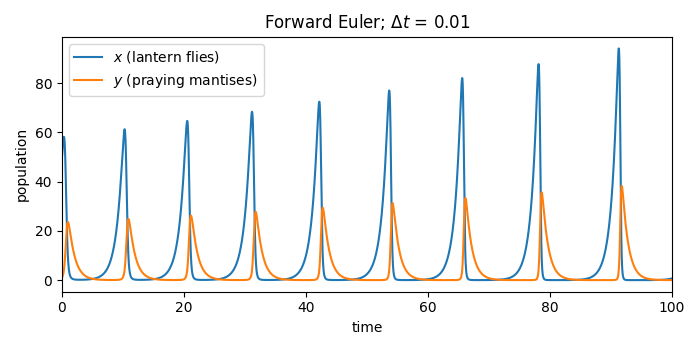
\includegraphics[width=0.8\textwidth]{lv_forward_euler.png}\\
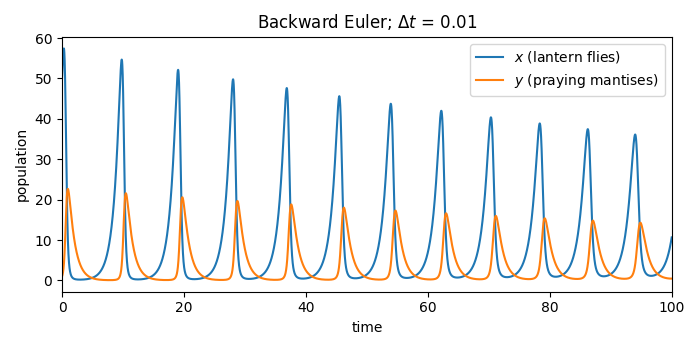
\includegraphics[width=0.8\textwidth]{lv_backward_euler.png}\\
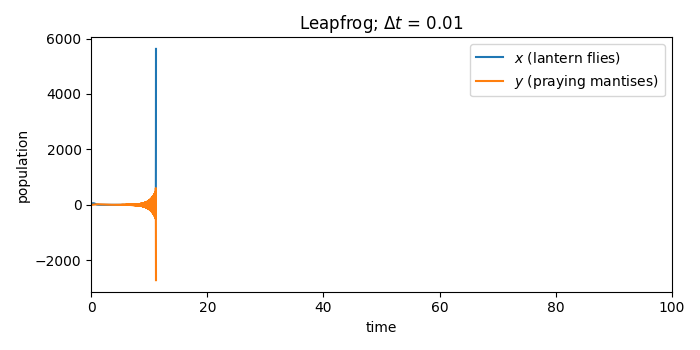
\includegraphics[width=0.8\textwidth]{lv_leapfrog.png}
\end{center}

g. Our original question concerns the stability behavior of the system.  What answer does each of the simulations suggest: lantern fly populations will blow up indefinitely, collapse and stabilize, or oscillate?  Do your simulations lead to the same answer and, if not, which one do you believe most likely reflects the stability behavior the model should exhibit if you could simulate it perfectly?  Justify your answer in a sentence or two.

{\color{red}
The forward Euler simulation grows in larger and larger peaks, suggesting the populations explode. The backward Euler simulation shrinks in smaller and smaller peaks, suggesting the population will eventually stabilize near our established equilibrium. The leapfrog simulation already diverges by $t \approx 11$, suggesting the populations explode too, but this comes from numerical instability (the populations even go negative) and is not a plausible event.

The simulations do not agree. I think the true model is something in-between: the populations oscillate around the equilibrium $(10, 4)$ forever with a constant amplitude. The model conserves $V = cx - d\ln x + by - a\ln y$ (one can check $dV/dt = 0$), so an exact solution stays on one closed orbit. Forward Euler pushes $V$ up every cycle and backward Euler pulls it down.
}

{\bf *Problem 5 (20 points):}  In this problem, we will look to develop a new numerical integration method.  Our goal will be to develop a version of the leapfrog method that works for variable step sizes.  That is, we will assume our previous step covered some time $\Delta t_1$ and we now want to take another step $\Delta t_2$, with the assumption that in general $\Delta t_1 \ne \Delta t_2$.  Our goal will be to derive a formula for a second derivative approximation combining $x(t-\Delta t_1)$, $x(t)$, and $x'(t)$ to derive $x(t+\Delta t_2)$.

a. First, we will need Taylor expansions of the terms around $t$.  Provide this for the $x(t-\Delta t_1)$ and $x(t+\Delta t_2)$ terms.  To derive second order approximations, we will want to truncate at with fourth order error terms.

\textcolor{red}{
$x(t - \Delta t_1) = x(t) - \Delta t_1 x'(t) + \frac{\Delta t_1^2}{2} x''(t) - \frac{\Delta t_1^3}{6} x'''(t) + O(\Delta t_1^4)$\\
$x(t + \Delta t_2) = x(t) + \Delta t_2 x'(t) + \frac{\Delta t_2^2}{2} x''(t) + \frac{\Delta t_2^3}{6} x'''(t) + O(\Delta t_2^4)$
}

b. Now, we will want to figure out what the coefficients should be for the terms to derive a consistent formula $ax(t-\Delta t_1) + bx(t) + cx'(t) \approx x(t+\Delta t_2)$.  Pose this as a linear systems problem.

{\color{red}
$ax(t - \Delta t_1) + b\, x(t) + c\, x'(t) \approx x(t + \Delta t_2)\\
\rightarrow \quad ax(t - \Delta t_1) + b\, x(t) + c\, x'(t) - x(t + \Delta t_2) = 0$
Substituting the Taylor expansions from part a and matching the coefficients of $x(t)$, $x'(t)$, and $x''(t)$:
\begin{align*}
x(t)&: & a + b - 1 = 0 \quad &\rightarrow \quad a + b = 1\\
x'(t)&: & -a\Delta t_1 + c - \Delta t_2 = 0 \quad &\rightarrow \quad -a\Delta t_1 + c = \Delta t_2\\
x''(t)&: & a \frac{\Delta t_1^2}{2} - \frac{\Delta t_2^2}{2} = 0 \quad &\rightarrow \quad a \Delta t_1^2 = \Delta t_2^2
\end{align*}
As a linear system:
\[\begin{pmatrix} 1 & 1 & 0 \\ -\Delta t_1 & 0 & 1 \\ \Delta t_1^2 & 0 & 0 \end{pmatrix}
\begin{pmatrix} a \\ b \\ c \end{pmatrix}
= \begin{pmatrix} 1 \\ \Delta t_2 \\ \Delta t_2^2 \end{pmatrix}\]
}

c. Solve for the coefficients for the scheme to give it as much accuracy as possible.

\textcolor{red}{
\[a = \frac{\Delta t_2^2}{\Delta t_1^2}\]
\[b = 1 - a = 1 - \frac{\Delta t_2^2}{\Delta t_1^2}\]
\[c = a\Delta t_1 + \Delta t_2 = \left(\frac{\Delta t_2^2}{\Delta t_1^2}\right)\Delta t_1 + \Delta t_2 = \frac{\Delta t_2^2}{\Delta t_1} + \Delta t_2 = \Delta t_2\left(1 + \frac{\Delta t_2}{\Delta t_1}\right)\]
This now results in the following:
$x(t + \Delta t_2) \approx \frac{\Delta t_2^2}{\Delta t_1^2}\, x(t - \Delta t_1) + \left(1 - \frac{\Delta t_2^2}{\Delta t_1^2}\right) x(t) + \Delta t_2\left(1 + \frac{\Delta t_2}{\Delta t_1}\right) x'(t)$
}

d. What order accuracy is the method we have derived?

\textcolor{red}{
Through Local Truncation Error, as we're matching everything through the second derivative, the first term we couldn't remove was the 3rd derivative term
\[-\frac{a \Delta t_1^3}{6} x'''(t) - \frac{\Delta t_2^3}{6} x'''(t) = -\frac{\Delta t_2^2 \Delta t_1 + \Delta t_2^3}{6} x'''(t)\]
Thus, the local error scales as $O(\Delta t^3)$. But this is only the error at a single step so to go into total error of the entire simulation, we should multiply it by the number of steps, $T/\Delta t$, which gives $\left( \frac{T}{\Delta t} \right) \cdot \Delta t^3 = T\,\Delta t^2$. That's our total global error and thus, this is second-order accurate.
}

{\bf *}Recall that the starred problems are only for the 02-712 students.


\end{document}